\documentclass[aspectratio=169, 14pt]{beamer}
\usepackage[utf8]{inputenc}
\usepackage[english]{babel}
\usepackage{xeCJK}
\xeCJKsetup{CJKmath=true}
\usepackage{amsmath}
\usepackage{graphicx}
\usepackage{transparent}
\usepackage[ruled, lined, linesnumbered, commentsnumbered]{algorithm2e}
\usepackage{tikz}
\usetikzlibrary{calc,shadows.blur}
\usetikzlibrary{matrix,backgrounds}
\usetikzlibrary{arrows, positioning}
\usetikzlibrary{arrows.meta}
\usepackage{minted}
\usepackage{fontawesome5}
\usepackage{booktabs}
\usepackage{caption}
\usepackage{hyperref}
\hypersetup{
    colorlinks=true,
    linkcolor=blue,
    filecolor=magenta,      
    urlcolor=cyan,
    }
\urlstyle{same}
\usetheme{metropolis}
\metroset{block=fill}
\usecolortheme{default}
\definecolor{darkmidnightblue}{rgb}{0.0, 0.2, 0.4}
\definecolor{LightGray}{gray}{0.9}

\usepackage{fontspec}

% mac
% \newfontfamily\suitfont{DejaVu Sans Mono Nerd Font Complete}
% manjaro
% \newfontfamily\suitfont{DejaVu Sans}
\usepackage{arev}
%------------------------------------------------------------
%This block of code defines the information to appear in the
%Title page
\title[Database Principles and Applications] %optional
{数据库原理与应用}

\subtitle{Relational Model}

\author[CHEN Zhongpu] % (optional)
{CHEN Zhongpu}

\institute[] % (optional)
{
  School of Computing and Artificial Intelligence \\
  \href{mailto:zpchen@swufe.edu.cn}{zpchen@swufe.edu.cn}
}

\date[] % (optional)
{SWUFE, Spring \the\year{}}

%End of title page configuration block
%------------------------------------------------------------


%------------------------------------------------------------
%The next block of commands puts the table of contents at the 
%beginning of each section and highlights the current section:

% \AtBeginSection[]
% {
%   \begin{frame}
%     \frametitle{Table of Contents}
%     \tableofcontents[currentsection]
%   \end{frame}
% }
%------------------------------------------------------------


\begin{document}

%The next statement creates the title page.
\frame{\titlepage}

%---------------------------------------------------------
%This block of code is for the table of contents after
%the title page
% \begin{frame}
% \frametitle{Table of Contents}
% \tableofcontents
% \end{frame}
%--------------------------------------------------------
\begin{frame}
	\frametitle{复习}
	\begin{block}{数据模型}
		数据模型 (data model) 描述数据、数据关系、数据语义和一致性约束的概念化工具的集合。
	\end{block}
	\begin{itemize}
		\item \alert{关系模型}
		\item 实体-联系模型
		\item 对象模型
		\item 半结构化模型
		\item ...
	\end{itemize}
\end{frame}

{
% \usebackgroundtemplate{\transparent{0.3}{\begin{picture}
%     
\includegraphics[height=0.7\paperheight]{cover}
% \end{picture}    
% }}
\usebackgroundtemplate{
	\tikz[overlay,remember picture]
	\node[opacity=0.3, at=(current page.south east),anchor=south east, yshift=2cm,xshift=4cm] {
		
\includegraphics[height=0.6\paperheight]{cover}};
}
\begin{frame}
	\section{\textcolor{darkmidnightblue}{1. 关系数据库}}
	\begin{quote}
		A relational database consists of a collection of \alert{tables}.
	\end{quote}
\end{frame}
}

\begin{frame}
	\frametitle{Relation}

	\begin{exampleblock}{Relation}
		Given sets $X$ and $Y$, the Cartesian product $X \times Y$ is defined as $\{(x, y) | x \in X \text{ and } y \in Y\}$, and its elements are called ordered pairs.

		A \alert{binary relation} $R$ over sets $X$ and $Y$ is a subset of $X \times Y$.
	\end{exampleblock}


\end{frame}
\begin{frame}
	\frametitle{1.1 关系数据库的结构}

	\begin{columns}
		\column{0.45\textwidth}
		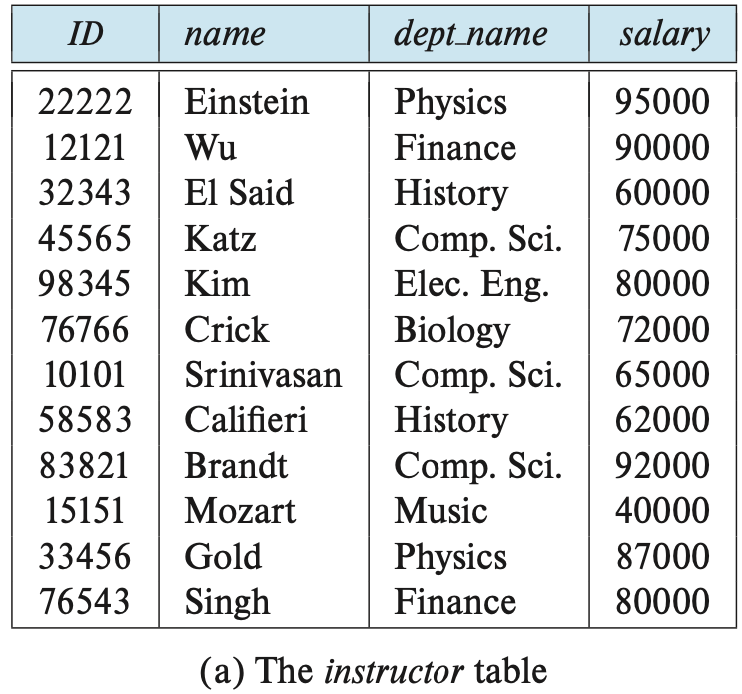
\includegraphics[width=\textwidth]{table/instructor}
		\column{0.55\textwidth}
		\begin{table}
			\begin{tabular}{ll}
				\toprule
				数据库                    & Excel      \\
				\midrule
				\alert{关系} (relation)  & 表 (table)  \\
				\alert{元组} (tuple)     & 行 (row)    \\
				\alert{属性} (attribute) & 列 (column) \\
				\bottomrule
			\end{tabular}
		\end{table}
		\begin{quote}
			A row in a table represents a \textbf{relationship} among a set of values.
		\end{quote}
	\end{columns}
\end{frame}
\begin{frame}
	\begin{figure}
		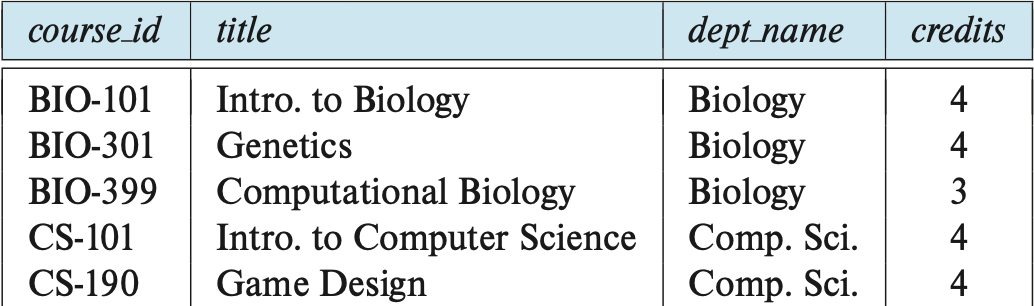
\includegraphics[height=.35\paperheight]{table/course}
		\caption*{The \emph{course} table}
	\end{figure}
	\begin{columns}
		\column{0.4\textwidth}
		\begin{figure}
			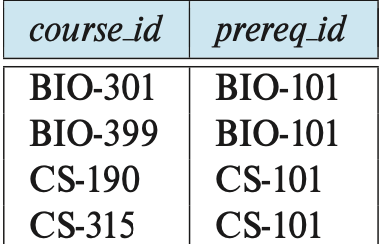
\includegraphics[height=.35\paperheight]{table/prereq}
			\caption*{The \emph{prereq} table}
		\end{figure}
		\column{0.575\textwidth}
		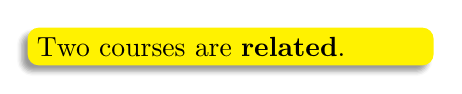
\begin{tikzpicture}
			\node[fill=yellow,blur shadow={shadow xshift=-0.5ex},
				text width=14em,anchor=south west,rounded corners]
			{Two courses are \textbf{related}.};
		\end{tikzpicture}
	\end{columns}
\end{frame}
\begin{frame}
	\frametitle{思考}
	\begin{block}{关系}
		关系 (relation) 是元组(tuple) 的集合 (set)。
	\end{block}

	\begin{columns}
		\column{0.4\textwidth}
		\begin{figure}
			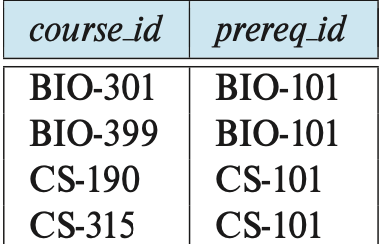
\includegraphics[height=.35\paperheight]{table/prereq}
			\caption*{The \emph{prereq} table}
		\end{figure}
		\column{0.6\textwidth}
		\begin{enumerate}
			\item 元组出现的顺序是否重要?
			\item 元组是否可以重复?
		\end{enumerate}
	\end{columns}

\end{frame}

\begin{frame}
	\frametitle{1.2 关系模式}
	\begin{itemize}
		\item 数据库模式 (database schema):数据库的逻辑设计
		\item 数据库实例 (database instance):给定时刻数据库中数据的快照
	\end{itemize}
	类似的,也有关系模式 (relation schema)和关系实例 (relation instance)。

	\begin{tikzpicture}
		\node[fill=yellow,blur shadow={shadow xshift=-0.5ex},
			text width=26em,anchor=south west,rounded corners]
		{很多参考资料中使用“关系”一词同时表示“关系模式”或“关系实例”。};
	\end{tikzpicture}
\end{frame}

\begin{frame}
	\begin{columns}
		\column{.5\textwidth}
		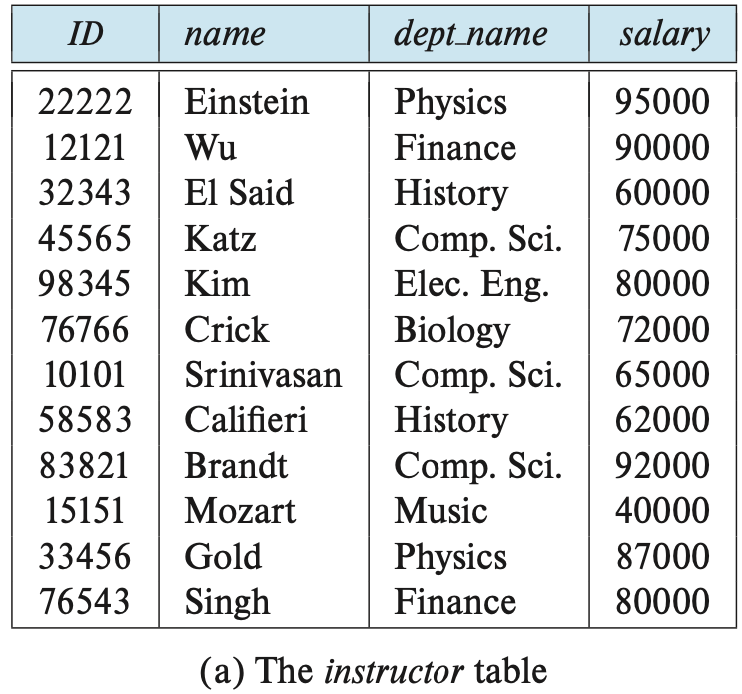
\includegraphics[height=.7\paperheight]{table/instructor}
		\column{.5\textwidth}
		The name of a relation and the set of attributes for a relation is called the \alert{schema} for that relation.
	\end{columns}
	\texttt{instructor(ID, name, dept\_name, salary)}
\end{frame}
\begin{frame}

	\begin{center}
		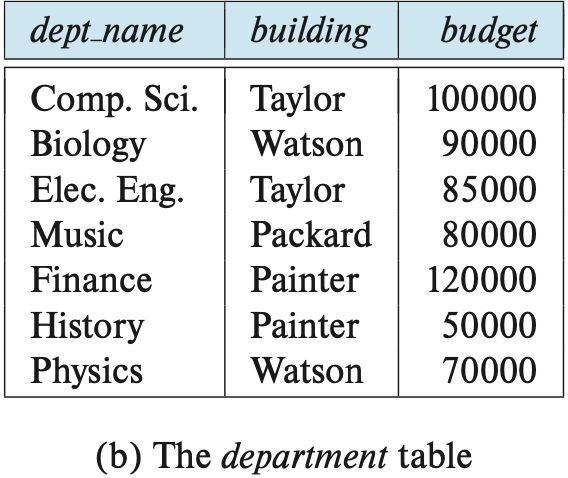
\includegraphics[height=.7\paperheight]{table/department}
	\end{center}
\end{frame}

\begin{frame}

	\begin{itemize}
		\item \texttt{\textbf{course}(course\_id, title, dept\_name, credits)}
		\item \texttt{\textbf{student}(ID, name, dept\_name, tot\_cred)}
		\item \texttt{\textbf{advisor}(s\_id, i\_id)}
		\item \texttt{\textbf{section}(course\_id, sec\_id, semester, year, building, room\_number, time\_slot id)}
		\item \texttt{\textbf{takes}(ID, course\_id, sec\_id, semester, year, grade)}
		\item \texttt{\textbf{teaches}(ID, course\_id, sec\_id, semester, year)}
		\item \texttt{\textbf{classroom}(building, room\_number, capacity)}
		\item \texttt{\textbf{time\_slot}(time\_slot\_id, day, start\_time, end\_time)}
	\end{itemize}

\end{frame}

\begin{frame}
	\section{\textcolor{darkmidnightblue}{2. 码 (key)}}
	
\includegraphics[height=.3\paperheight]{image/census}
\end{frame}

\begin{frame}
	\frametitle{人口普查系统}
	\begin{table}
		\begin{tabular}{llll}
			\toprule
			名字 & 年龄 & 籍贯 & 民族 \\
			\midrule
			张伟 & 25 & 安徽 & 汉  \\
			\bottomrule
		\end{tabular}
	\end{table}
	{\large \faIcon[regular]{lightbulb}} 如何区分重名的数据?

	\begin{tikzpicture}
		\node[fill=blue!20,blur shadow={shadow xshift=-0.5ex},
			text width=26em,anchor=south west,rounded corners]
		{全国有近30万个“张伟”;名为“王伟”“李娜”的人数紧随其后,均超过27万人。};
	\end{tikzpicture}
\end{frame}

\begin{frame}
	\frametitle{2.1 码 (key)}
	\begin{exampleblock}{码}
		一种区分给定「关系」中的不同「元组」的方法。
	\end{exampleblock}

	\begin{table}
		\caption*{people}
		\begin{tabular}{lllll}
			\toprule
			name & age & origin & nationality & id      \\
			\midrule
			张伟   & 25  & 安徽     & 汉           & 3408xxx \\
			\bottomrule
		\end{tabular}
	\end{table}
	\texttt{people(name, age, origin, nationality, id)}
\end{frame}

\begin{frame}
	\frametitle{2.2 超码 (super key)}
	\begin{exampleblock}{超码}
		一个或多个属性的集合,这样属性的组合可以使我们在一个关系中唯一地标识一个元组。
	\end{exampleblock}
	\textcolor{red}{\texttt{people(name, age, origin, nationality, id)}}
	\pause
	\begin{columns}
		\column{0.4\textwidth}
		\begin{itemize}
			\item \texttt{(id)}
			\item \texttt{(id, name)}
			\item \texttt{(id, age)}
			\item \texttt{(id, name, age)}
			\item ...
		\end{itemize}
		\column{0.5\textwidth}
		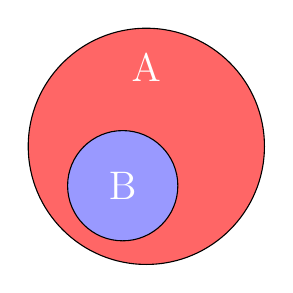
\begin{tikzpicture}
			\draw[fill=red!60] (0,0) circle(1.5cm);
			\draw[fill=blue!40] (-0.3, -0.5) circle(0.7cm);
			\node[white] at (0, 1) {\Large A};
			\node[white] at (-0.3, -0.5) {\Large B};
		\end{tikzpicture}
	\end{columns}
\end{frame}
\begin{frame}
	\frametitle{2.3 候选码 (candidate key)}
	\begin{exampleblock}{候选码}
		其真子集不能构成超码的超码 (又称“最小超码”)。
	\end{exampleblock}
	\begin{columns}
		\column{0.45\textwidth}<1->
		\begin{itemize}
			\item \texttt{(id)}
			\item \texttt{(id, name)}
			\item \texttt{(id, age)}
			\item ...
		\end{itemize}
		{\large \faIcon[regular]{lightbulb}} \textbf{思考}:候选码是否唯一?
		\column{0.55\textwidth}<2->
		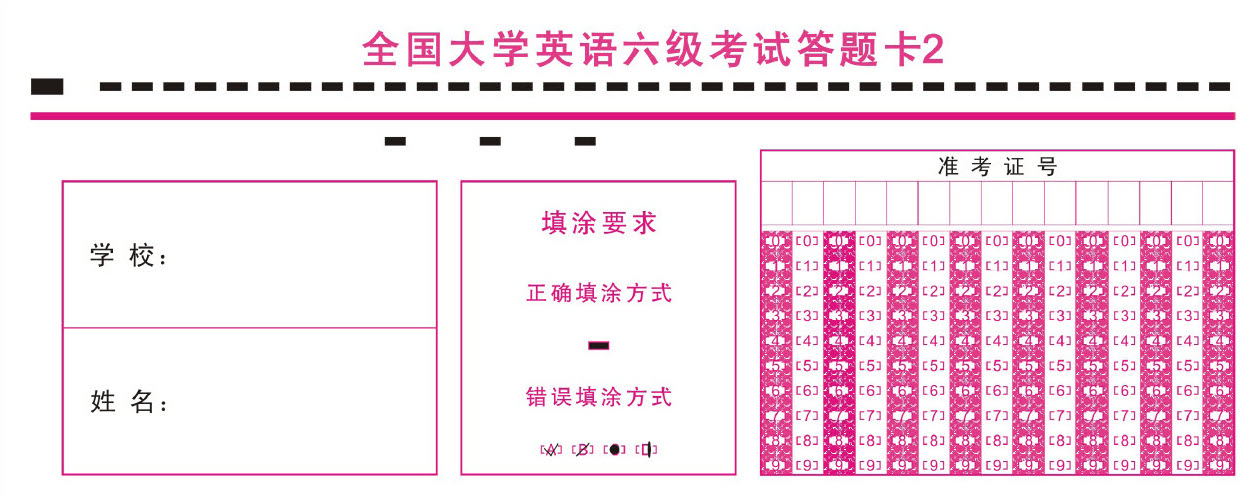
\includegraphics[width=\textwidth, trim={0 14cm 0 0},clip]{image/exam}
	\end{columns}

\end{frame}

\begin{frame}
	\frametitle{2.4 主码 (primary key)}
	\begin{exampleblock}{主码}
		被数据库设计者选中的候选码。
	\end{exampleblock}

	\texttt{people(name, age, origin, nationality, \underline{id})}

\end{frame}

\begin{frame}
	\frametitle{练习 {\large \faIcon{code}}}
	\textbf{练习一}:人口普查 people 关系中住址 (address) 能否作为主码?
	\noindent\rule{\textwidth}{1pt}
	\textbf{练习二}:考虑大学中的classroom 关系,classroom (building, room\_number, capacity),其主码是什么?
\end{frame}

\begin{frame}
	\begin{center}
		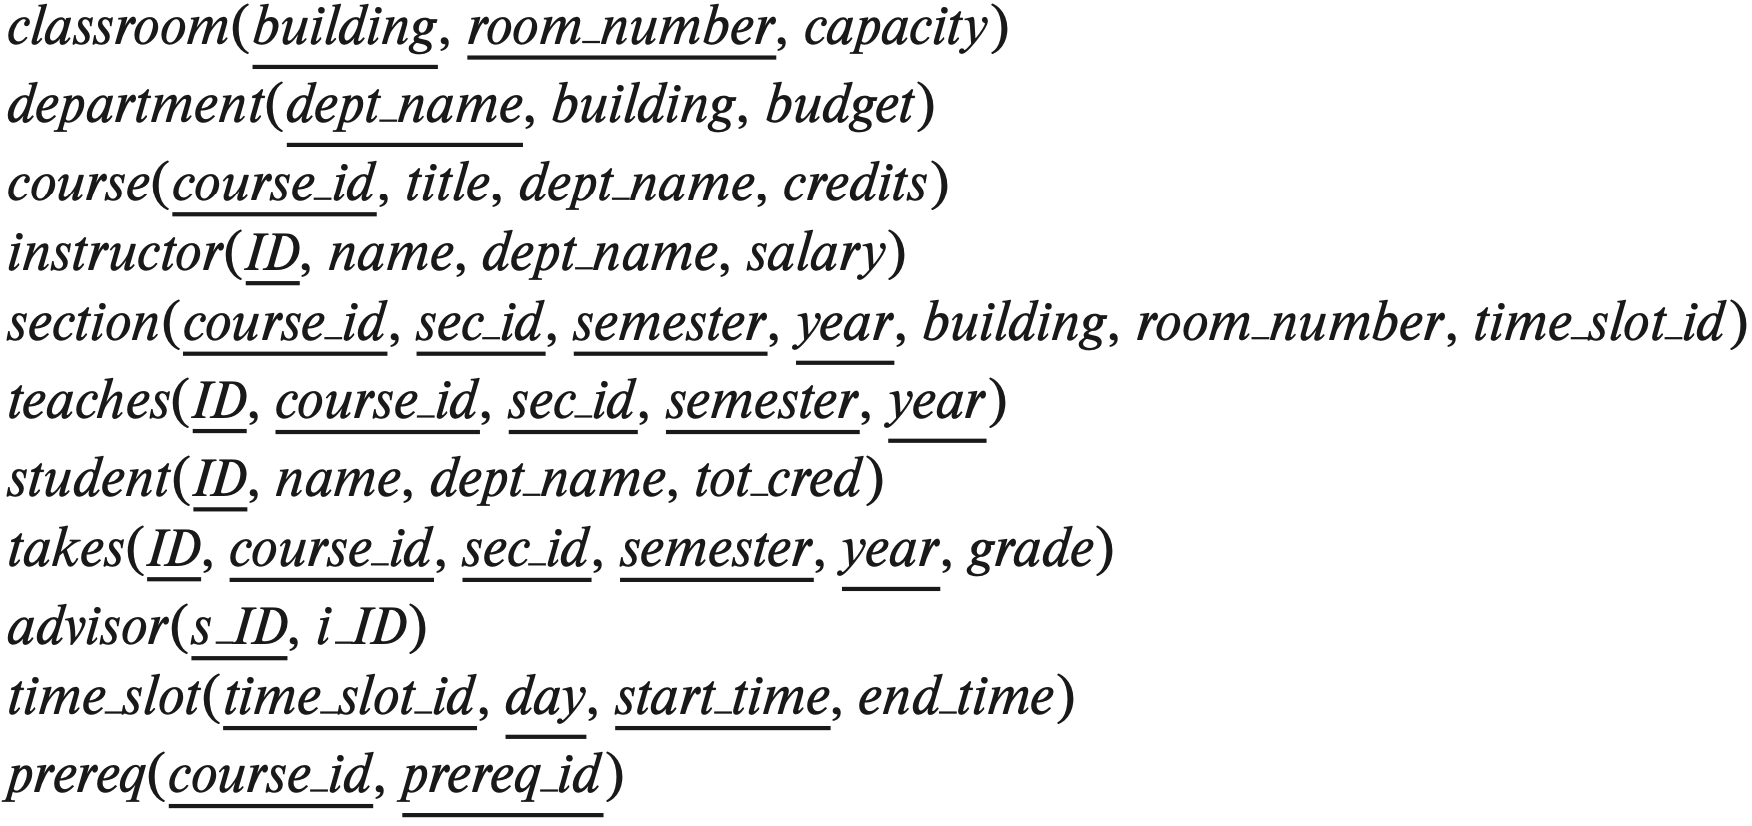
\includegraphics[height=.75\paperheight]{table/schema}
	\end{center}

\end{frame}

\begin{frame}
	\frametitle{2.5 外码 (foreign key)}

	\begin{quote}
		Attribute \texttt{dept\_name} is a \alert{foreign key} from \texttt{instructor}, referencing \texttt{department}.
	\end{quote}


	\begin{itemize}
		\item \alert{参照关系} (referencing relation):\texttt{\textbf{instructor}(\underline{ID}, name, dept\_name, salary)}
		\item  \alert{被参照关系} (referenced relation):
		      \texttt{\textbf{department}(\underline{dept\_name}, building, budget)}
	\end{itemize}

	\begin{tikzpicture}
		\node[fill=yellow,blur shadow={shadow xshift=-0.5ex},
			text width=26em,anchor=south west,rounded corners]
		{注意:外码与其所参照关系的主码的名字不一定相同。};
	\end{tikzpicture}
\end{frame}

\begin{frame}
	\section{\textcolor{darkmidnightblue}{3. 关系代数 (relation algebra)}}
	关系代数是 SQL 的理论基础
\end{frame}

\begin{frame}
	\frametitle{什么是关系代数}
	\begin{quote}
		Algebra is the study of mathematical symbols and the rules for manipulating these symbols.
		代数是对数学符号以及操纵这些符号的规则的研究。
	\end{quote}

	\[x = \frac{-b \pm \sqrt{b^2 - 4ac}}{2a}\]

	\begin{tikzpicture}
		\node[fill=yellow,blur shadow={shadow xshift=-0.5ex},
			text width=26em,anchor=south west,rounded corners]
		{关系代数是定义在\alert{关系、元组和属性}上的操作。};
	\end{tikzpicture}

\end{frame}

\begin{frame}
	\frametitle{为什么需要学习关系代数}
	虽然商业数据库基本都是采用 SQL,而不是直接使用关系代数,但是当 DBMS 执行查询的时候,它做的第一件事就是\textbf{将 SQL 翻译成关系代数(或者其他类似的表示)}。


	关系代数有用的第二个原因是:\textbf{相较其他通用的编程语言(如C、Java),它不够强大}。它仅提供有限的操作,从而便于查询编译器能够产生优化的代码。

\end{frame}

\begin{frame}[fragile]
	\frametitle{3.1 关系代数}

	\begin{columns}
		\column{.475\textwidth}
		\begin{tikzpicture}[slot/.style={minimum size=1.4cm,rectangle}, relation/.style={slot, fill=black!30},operation/.style={circle, fill=blue!30},>=Stealth]
			\matrix [nodes=draw, row sep=0.2cm, column sep=1cm] {
				\node[relation](t1) {关系};              & \node[operation](o1) {操作}; & \node[relation](t2) {关系};  \\
				\node[relation, yshift=-1cm](ta) {关系}; &                            &                            \\
				                                       & \node[operation](o2) {操作}; & \node[relation] (t3) {关系}; \\
				\node[relation](tb){关系};               &                            &                            \\
			};

			\draw[->, thick] (t1) -- (o1);
			\draw[->, thick] (o1) -- (t2);
			\draw[->, thick] (ta) -- (o2);
			\draw[->, thick] (tb) -- (o2);
			\draw[->, thick] (o2) -- (t3);
		\end{tikzpicture}
		\column{.475\textwidth}
		\begin{tikzpicture}
			\node[fill=yellow,blur shadow={shadow xshift=-0.5ex},
				text width=14em,anchor=south west,rounded corners]
			{运算要么施加于单个关系上,要么施加于两个关系。\textbf{运算结果总是单个关系}。};
		\end{tikzpicture}
	\end{columns}
\end{frame}

\begin{frame}
	\frametitle{选择 (select)}

	\begin{columns}
		\column{.475\textwidth}
		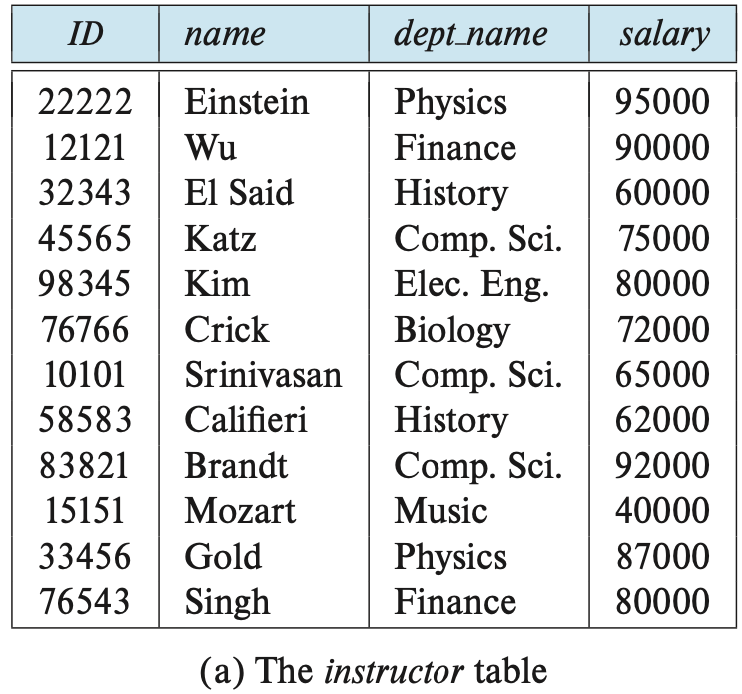
\includegraphics[width=\textwidth]{table/instructor}
		\column{.475\textwidth}
		\alert{选择} \texttt{dept\_name} 为 \texttt{Physics}的所有老师。
		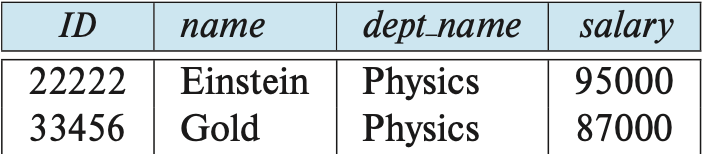
\includegraphics[width=\textwidth]{table/select-instructor}

		\begin{tikzpicture}
			\node[fill=yellow,blur shadow={shadow xshift=-0.5ex},
				text width=10em,anchor=south west,rounded corners]
			{小写希腊字母sigma};
		\end{tikzpicture}

	\end{columns}
	\pause
	\large{\[\sigma_{dept\_name =  ``Physics"}(instructor)\]}

\end{frame}

\begin{frame}

	\begin{columns}
		\column{.475\textwidth}
		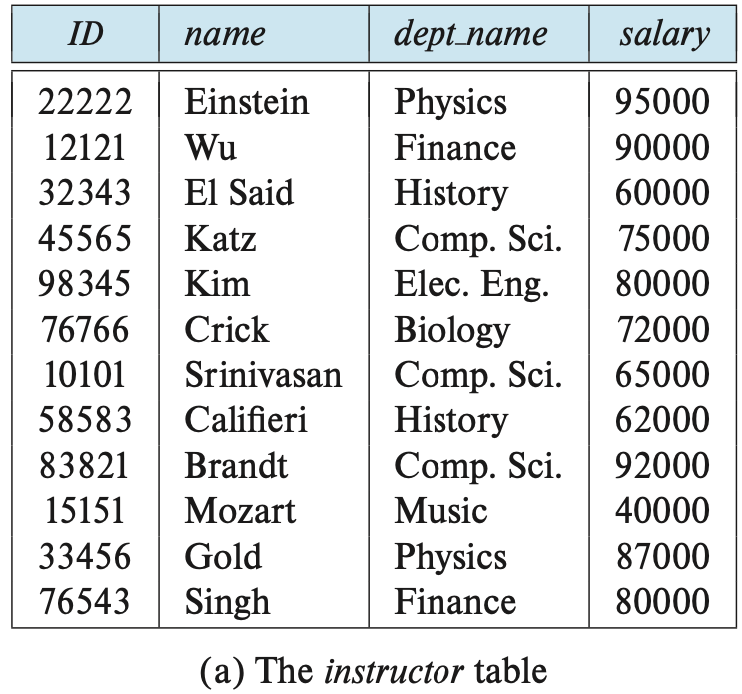
\includegraphics[width=\textwidth]{table/instructor}
		\column{.475\textwidth}
		\alert{选择} \texttt{salary} 大于 90000 的所有老师。
		\large{\[\sigma_{salary >  90000}(instructor)\]}
	\end{columns}

\end{frame}

\begin{frame}
	谓词(predicate)的比较操作可以使用符号:$>$, $<$, $=$, $\geq$, $\leq$, $\neq$。此外,多个谓词可以通过\alert{逻辑联结词} (logical connectives)结合:

	\begin{itemize}
		\item and: $\land$
		\item or: $\lor$
		\item not: $\neg$
	\end{itemize}

	\pause

	{\large \faIcon{code}} \textbf{练习}:选择在 Physics 学院且 salary 大于 90000 的所有老师。

\end{frame}

\begin{frame}
	\frametitle{投影 (project)}
	返回所有老师的 \texttt{name}、\texttt{dept\_name} 和 \texttt{salary}。
	\begin{columns}
		\column{.475\textwidth}
		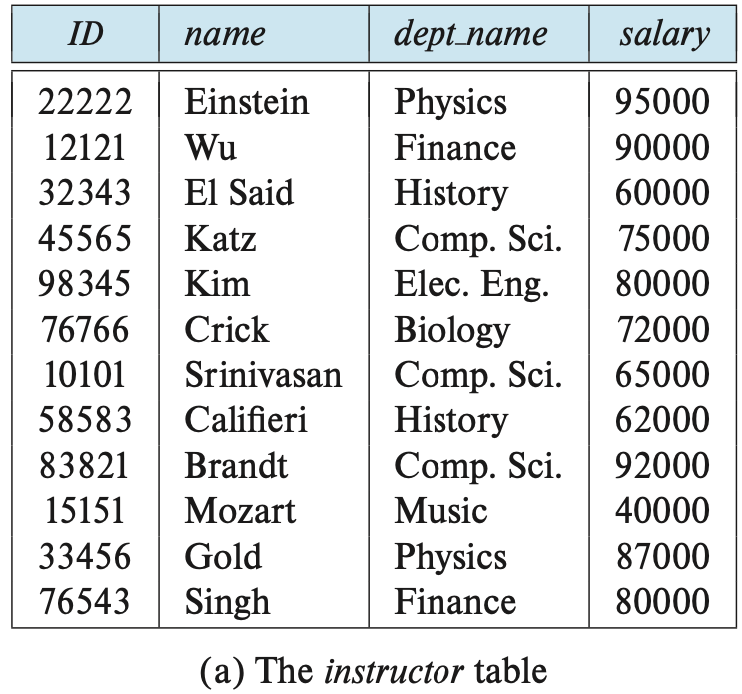
\includegraphics[width=\textwidth, trim={0 4.4cm 0 0},clip]{table/instructor}
		\column{.475\textwidth}
		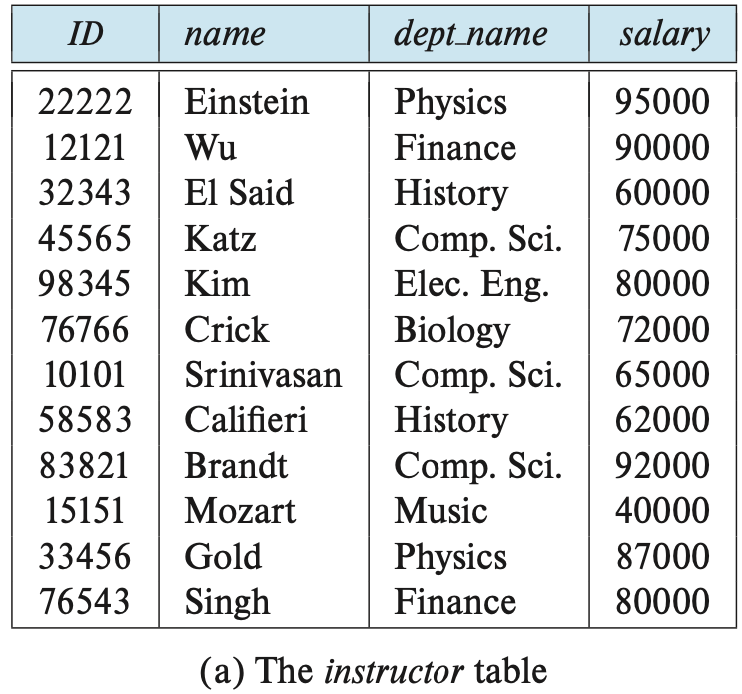
\includegraphics[height=.4\paperheight, trim={2.8cm 4.4cm 0 0},clip]{table/instructor}
		\pause
		\begin{tikzpicture}
			\node[fill=yellow,blur shadow={shadow xshift=-0.5ex},
				text width=8em,anchor=south west,rounded corners]
			{大写希腊字母Pi};
		\end{tikzpicture}
	\end{columns}
	\large{\[\Pi_{ID, dept\_name, salary}(instructor)\]}
\end{frame}

\begin{frame}
	\begin{center}
		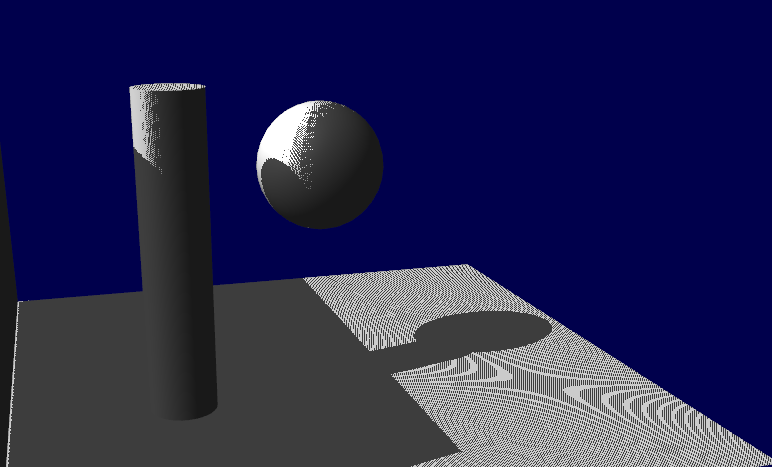
\includegraphics[width=.45\textwidth]{image/project}
	\end{center}

	\begin{itemize}
		\item select ($\sigma$):\alert{水平地}截取关系,影响「行」
		\item project ($\Pi$):\alert{垂直地}截取关系,影响「列」
	\end{itemize}
	\pause
	并且,通用的投影操作允许在属性上进行简单的运算:\large{\(\Pi_{ID, name, salary/12}(instructor)\)}

\end{frame}

\begin{frame}
	\frametitle{关系运算的组合}
	找出所有 Physics 学院老师的 name。
	{\large \[\Pi_{name}(\sigma_{dept\_name=``Physics"}(instructor))\]}
	\begin{center}
		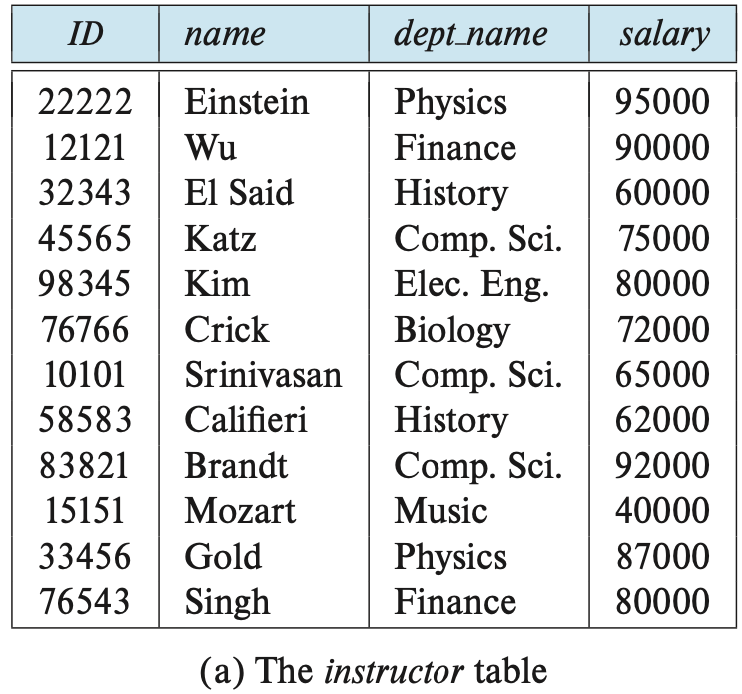
\includegraphics[width=.55\textwidth, trim={0 4.4cm 0 0},clip]{table/instructor}
	\end{center}

\end{frame}

\begin{frame}
	\frametitle{笛卡尔积 (Cartesian product)}
	\[A \times B = \{(a, b): a \in A, b \in B\}\]
	\pause
	\begin{itemize}
		\item $\varheart\vardiamond\clubsuit\spadesuit$
		\item \{A, K, Q, J, 10, 9, 8, 7, 6, 5, 4, 3, 2\}
	\end{itemize}
	{\large \faIcon{question-circle}} 一副牌一共有多少张?

	\pause
	\begin{itemize}
		\item \texttt{instructor(ID, name, dept\_name, salary)}
		\item \texttt{teaches(ID, course\_id, sec\_id, semester, year)}
	\end{itemize}
\end{frame}

\begin{frame}

	$r = instructor \times teaches$的关系模式可以写成:
	\begin{equation*}
		\begin{split}
			r(instructor.ID, name, dept\_name, salary, teaches.ID, \\ course\_id, sec\_id, semester, year)
		\end{split}
	\end{equation*}

	\begin{figure}
		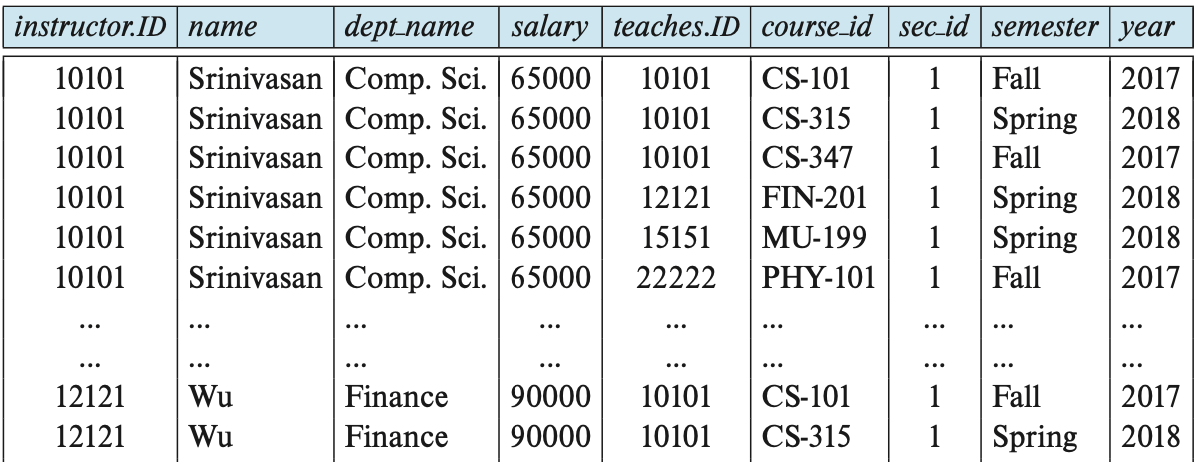
\includegraphics[width=.8\textwidth]{table/join}
		\caption*{$r = instructor \times teaches$}
	\end{figure}
\end{frame}

\begin{frame}
	\frametitle{连接 (join)}
	\begin{figure}
		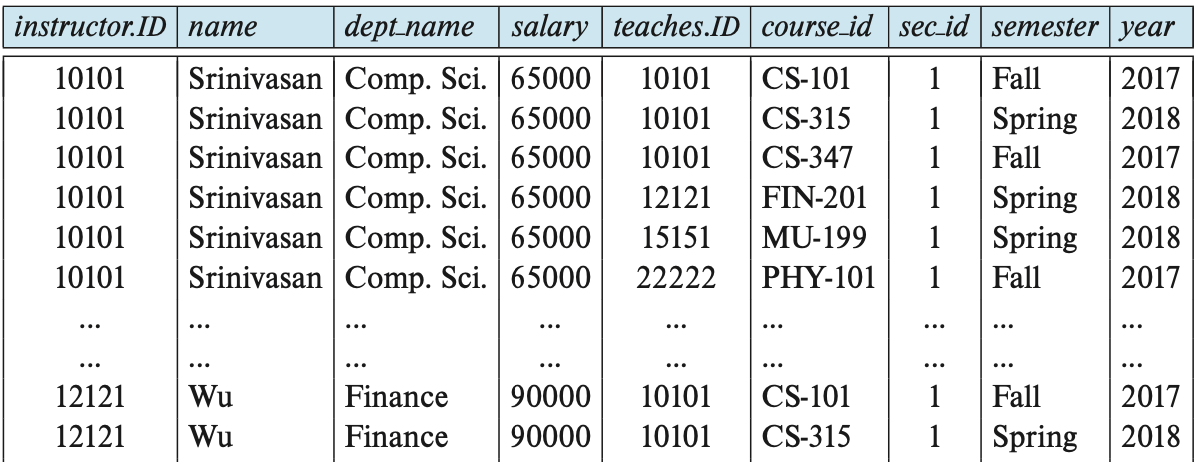
\includegraphics[width=.6\textwidth]{table/join}
		\caption*{$r = instructor \times teaches$}
	\end{figure}
	找出所有老师及其上课的信息:
	{\large \[\sigma_{instructor.ID=teaches.ID}(instructor \times teaches)\]}
\end{frame}

\begin{frame}
	\texttt{join}是笛卡尔积 (Cartesian product) 和选择 (selection) 的结合:
	{\large \[instructor \Join_{instructor.ID=teaches.ID} teaches\]}
	\begin{figure}
		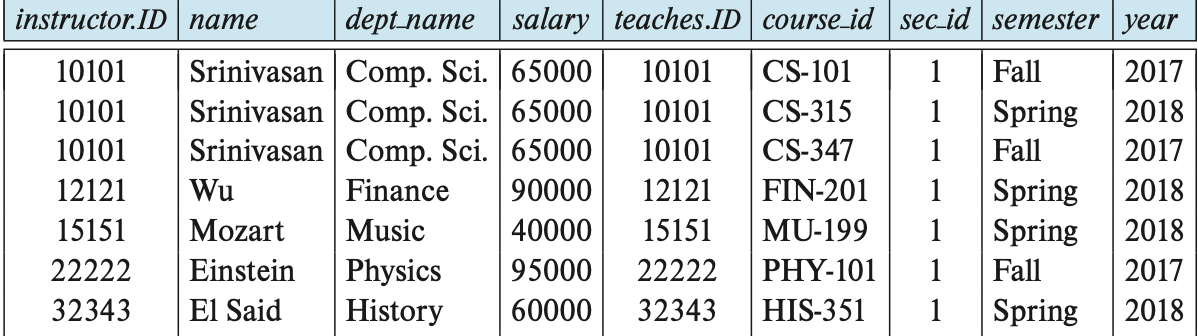
\includegraphics[width=.6\textwidth]{table/join2}
	\end{figure}

	\begin{exampleblock}{Join}
		考虑关系$r(R)$ 和 $s(S)$, $\theta$是关于属性$R \cup S$的一个谓词,连接操作$r \Join_{\theta} s= \sigma_{\theta}(r \times s)$
	\end{exampleblock}
\end{frame}

\begin{frame}
	\frametitle{自然连接 (natural join)}
	\begin{itemize}
		\item \texttt{instructor(ID, name, dept\_name, salary)}
		\item \texttt{teaches(ID, course\_id, sec\_id, semester, year)}
	\end{itemize}

	如果 $\theta$ 条件是\textbf{相同名称的属性值相等},就可以省略不写。此时叫\alert{自然连接}。
	{\large \[instructor \Join teaches \]}

\end{frame}

\begin{frame}
	\frametitle{并 (union)、交 (intersect)、差 (difference)}

	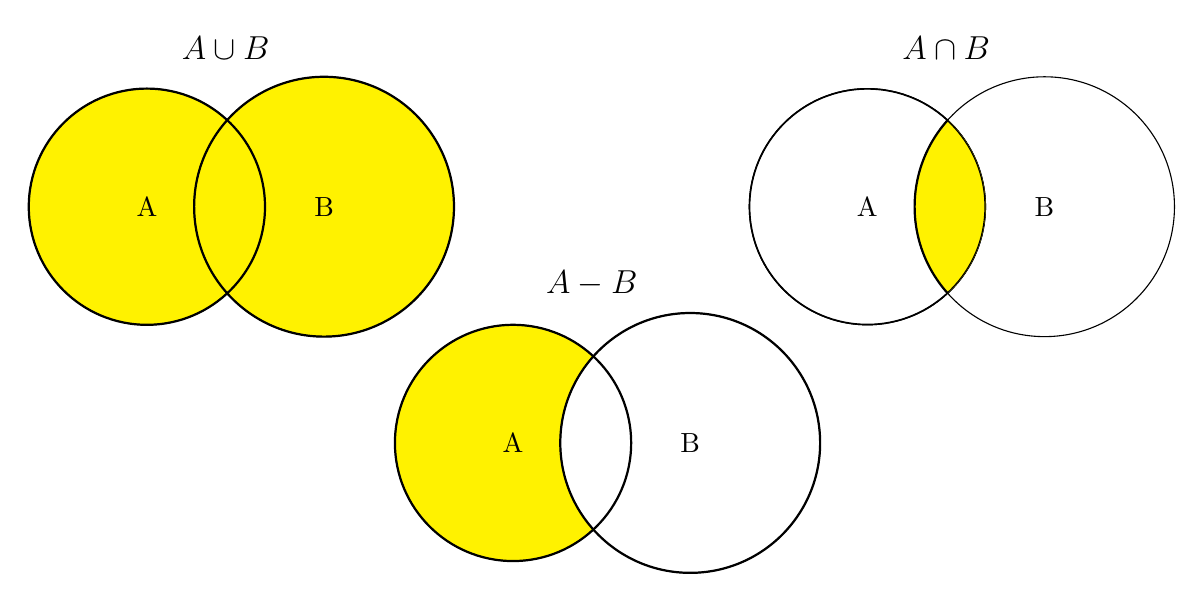
\begin{tikzpicture}[scale=0.75][thick]

		\begin{scope}[local bounding box=scope1]
			\draw [fill=yellow](0,0) circle (2cm);
			\draw [fill=yellow](3,0) circle (2.2cm);
			\draw[black,thick] (0,0) circle(2cm);
			\draw[black,thick] (3,0) circle(2.2cm);
			\draw (0,0) node(1a) {A};
			\draw (3,0) node {B};
		\end{scope}
		\node[above=of 1a, yshift=0.5cm, xshift=1cm] {\large $A \cup B$};
		\begin{scope}[shift={($(scope1.east)+(7cm,0)$)}]
			\draw (0,0) circle (2cm);
			\draw (3,0) circle (2.2cm);
			\draw (0,0) node(2a) {A};
			\draw (3,0) node {B};
			\draw [clip](0,0) circle (2cm);
			\fill[yellow] (3,0) circle (2.2cm);
			\draw[black,thick] (0,0) circle(2cm);
			\draw[black,thick] (3,0) circle(2.2cm);

		\end{scope}
		\node[above=of 2a, yshift=0.5cm, xshift=1cm] {\large $A \cap B$};

		\begin{scope}[shift={($(scope1.east)+(1cm,-4cm)$)}]
			\draw[fill=yellow] (0,0) circle (2cm);
			\draw[fill=white] (3,0) circle (2.2cm);
			\draw[black,thick] (0,0) circle(2cm);
			\draw[black,thick] (3,0) circle(2.2cm);
			\draw (0,0) node(3a) {A};
			\draw (3,0) node {B};
		\end{scope}
		\node[above=of 3a, yshift=0.5cm, xshift=1cm] {\large $A - B$};
	\end{tikzpicture}

\end{frame}

\begin{frame}
	\texttt{\textbf{section}(course\_id, sec\_id, semester, year, building, room\_number, time\_slot\_id)}

	找出所有同时在 2017 年 Fall 学期和 2018 年 Spring 学期的课程:

	\begin{equation*}
		\begin{split}
			\Pi_{course\_id}\bigl(\sigma_{semester=``Fall" \land year=2017}(section)\bigr) \\ \cap
			\Pi_{course\_id}\bigl(\sigma_{semester=``Spring" \land year=2018}(section)\bigr)
		\end{split}
	\end{equation*}

\end{frame}

\begin{frame}

	{\large \faIcon[regular]{lightbulb}} \textbf{思考}:\texttt{instructor} 和 \texttt{teaches} 的并、交、差是否有意义?

	\begin{itemize}
		\item \texttt{instructor(ID, name, dept\_name, salary)}
		\item \texttt{teaches(ID, course\_id, sec\_id, semester, year)}
	\end{itemize}
	\pause
	\begin{tikzpicture}
		\node[fill=yellow,blur shadow={shadow xshift=-0.5ex},
			text width=28em,anchor=south west,rounded corners]
		{两个关系进行并交差运算的前提是它们是\alert{相容的} (compatible),即两个关系的目 (arity) 相同,且每个对应属性的类型也相同。};
	\end{tikzpicture}
\end{frame}

\begin{frame}
	\frametitle{为什么要学关系代数?}
	\textbf{How important is it to understand spelling and grammar to be a writer? How important is it to understand history and law to be a politician? How important is it to understand chemistry to be pharmacist? How important is it to understand color theory to be an artist?}

	\emph{You can actually be a database developer, or any of these other jobs, if you haven't studied the theory behind the work, but you'll be limited to doing what you've seen before.}

\end{frame}

\begin{frame}
	\section{\textcolor{darkmidnightblue}{总结}}
	\begin{enumerate}
		\item 关系模式
		\item 超码、候选码、主码、外码
		\item 关系代数
	\end{enumerate}

\end{frame}

\begin{frame}
	\frametitle{练习 {\large \faIcon{code}}}
	\begin{itemize}
		\item \texttt{employee(\underline{ID}, person\_name, street, city)}
		\item \texttt{works(\underline{ID}, company\_name, salary)}
		\item  \texttt{company(\underline{company\_name}, city)}
	\end{itemize}

	\begin{enumerate}
		\item 找到所有居住在上海的员工的名字。
		\item 找到所有工资大于10000元的员工的名字。
	\end{enumerate}
\end{frame}

\begin{frame}
	\begin{itemize}
		\item \texttt{employee(\underline{ID}, person\_name, street, city)}
		\item \texttt{works(\underline{ID}, company\_name, salary)}
		\item  \texttt{company(\underline{company\_name}, city)}
	\end{itemize}

	\begin{enumerate}
		\item 找到所有居住在上海的员工的名字。
		      \[\Pi_{person\_name}(\sigma_{city=``上海"}(employee))\]
		\item 找到所有工资大于10000元的员工的名字。
		      \[\Pi_{person\_name}(\sigma_{salary>10000}(employee \Join work))\]
	\end{enumerate}

\end{frame}

\begin{frame}
	\frametitle{Homework 1}
	\href{https://github.com/ChenZhongPu/db-swufe/tree/master/02\_relational\_model}{02. Relational Model}

\end{frame}

\end{document}
